\documentclass[journal,12pt,twocolumn]{IEEEtran}
%
\usepackage{setspace}
\usepackage{gensymb}
%\doublespacing
\singlespacing

%\usepackage{graphicx}
%\usepackage{amssymb}
%\usepackage{relsize}
\usepackage[cmex10]{amsmath}
\usepackage{siunitx}
%\usepackage{amsthm}
%\interdisplaylinepenalty=2500
%\savesymbol{iint}
%\usepackage{txfonts}
%\restoresymbol{TXF}{iint}
%\usepackage{wasysym}
\usepackage{amsthm}
%\usepackage{iithtlc}
\usepackage{mathrsfs}
\usepackage{txfonts}
\usepackage{stfloats}
\usepackage{steinmetz}
\usepackage{supertabular}
%\usepackage{bm}
\usepackage{cite}
\usepackage{cases}
\usepackage{subfig}
%\usepackage{xtab}
\usepackage{longtable}
\usepackage{multirow}
%\usepackage{algorithm}
%\usepackage{algpseudocode}
\usepackage{enumitem}
\usepackage{mathtools}
\usepackage{tikz}
\usepackage{circuitikz}
\usepackage{verbatim}
\usepackage{tfrupee}
\usepackage[breaklinks=true]{hyperref}
%\usepackage{stmaryrd}
\usepackage{tkz-euclide} % loads  TikZ and tkz-base
%\usetkzobj{all}
\usepackage{pgfplots}
%\usetikzlibrary{all}
\usetikzlibrary{calc,math}
\usetikzlibrary{fadings}
\usetikzlibrary{automata, positioning, arrows}
\usepackage{listings}
    \usepackage{color}                                            %%
    \usepackage{array}                                            %%
    \usepackage{longtable}                                        %%
    \usepackage{calc}                                             %%
    \usepackage{multirow}                                         %%
    \usepackage{hhline}                                           %%
    \usepackage{ifthen}                                           %%
  %optionally (for landscape tables embedded in another document): %%
    \usepackage{lscape}     
\usepackage{multicol}
\usepackage{chngcntr}
\usepackage{blkarray}
%\usepackage{enumerate}

%\usepackage{wasysym}
%\newcounter{MYtempeqncnt}
\DeclareMathOperator*{\Res}{Res}
%\renewcommand{\baselinestretch}{2}
\renewcommand\thesection{\arabic{section}}
\renewcommand\thesubsection{\thesection.\arabic{subsection}}
\renewcommand\thesubsubsection{\thesubsection.\arabic{subsubsection}}

\renewcommand\thesectiondis{\arabic{section}}
\renewcommand\thesubsectiondis{\thesectiondis.\arabic{subsection}}
\renewcommand\thesubsubsectiondis{\thesubsectiondis.\arabic{subsubsection}}

% correct bad hyphenation here
\hyphenation{op-tical net-works semi-conduc-tor}
\def\inputGnumericTable{}                                 %%

\lstset{
%language=C,
frame=single, 
breaklines=true,
columns=fullflexible
}
%\lstset{
%language=tex,
%frame=single, 
%breaklines=true
%}

\begin{document}
%


\newtheorem{theorem}{Theorem}[section]
\newtheorem{problem}{Problem}
\newtheorem{proposition}{Proposition}[section]
\newtheorem{lemma}{Lemma}[section]
\newtheorem{corollary}[theorem]{Corollary}
\newtheorem{example}{Example}[section]
\newtheorem{definition}[problem]{Definition}
%\newtheorem{thm}{Theorem}[section] 
%\newtheorem{defn}[thm]{Definition}
%\newtheorem{algorithm}{Algorithm}[section]
%\newtheorem{cor}{Corollary}
\newcommand{\BEQA}{\begin{eqnarray}}
\newcommand{\EEQA}{\end{eqnarray}}
\newcommand{\define}{\stackrel{\triangle}{=}}

\bibliographystyle{IEEEtran}
%\bibliographystyle{ieeetr}


\providecommand{\mbf}{\mathbf}
\providecommand{\pr}[1]{\ensuremath{\Pr\left(#1\right)}}
\providecommand{\qfunc}[1]{\ensuremath{Q\left(#1\right)}}
\providecommand{\sbrak}[1]{\ensuremath{{}\left[#1\right]}}
\providecommand{\lsbrak}[1]{\ensuremath{{}\left[#1\right.}}
\providecommand{\rsbrak}[1]{\ensuremath{{}\left.#1\right]}}
\providecommand{\brak}[1]{\ensuremath{\left(#1\right)}}
\providecommand{\lbrak}[1]{\ensuremath{\left(#1\right.}}
\providecommand{\rbrak}[1]{\ensuremath{\left.#1\right)}}
\providecommand{\cbrak}[1]{\ensuremath{\left\{#1\right\}}}
\providecommand{\lcbrak}[1]{\ensuremath{\left\{#1\right.}}
\providecommand{\rcbrak}[1]{\ensuremath{\left.#1\right\}}}
\theoremstyle{remark}
\newtheorem{rem}{Remark}
\newcommand{\sgn}{\mathop{\mathrm{sgn}}}
\providecommand{\abs}[1]{\left\vert#1\right\vert}
\providecommand{\res}[1]{\Res\displaylimits_{#1}} 
\providecommand{\norm}[1]{\left\lVert#1\right\rVert}
%\providecommand{\norm}[1]{\lVert#1\rVert}
\providecommand{\mtx}[1]{\mathbf{#1}}
\providecommand{\mean}[1]{\text{E}\left( #1 \right)}
\providecommand{\var}[1]{\text{var}\left( #1 \right)}
\providecommand{\cov}[1]{\text{cov}\left( #1 \right)}
\providecommand{\fourier}{\overset{\mathcal{F}}{ \rightleftharpoons}}
\providecommand{\gauss}[2]{\ensuremath{\mathcal{N}\left({#1}, {#2} \right)}}
%\mathcal{N}\left(0,\frac{1}{4}\right)\\
%\providecommand{\hilbert}{\overset{\mathcal{H}}{ \rightleftharpoons}}
\providecommand{\system}{\overset{\mathcal{H}}{ \longleftrightarrow}}
	%\newcommand{\solution}[2]{\textbf{Solution:}{#1}}
\newcommand{\solution}{\noindent \textbf{Solution: }}
\newcommand{\cosec}{\,\text{cosec}\,}
\providecommand{\dec}[2]{\ensuremath{\overset{#1}{\underset{#2}{\gtrless}}}}
\newcommand{\myvec}[1]{\ensuremath{\begin{pmatrix}#1\end{pmatrix}}}
\newcommand{\mydet}[1]{\ensuremath{\begin{vmatrix}#1\end{vmatrix}}}
\newcommand*{\permcomb}[4][0mu]{{{}^{#3}\mkern#1#2_{#4}}}
\newcommand*{\perm}[1][-3mu]{\permcomb[#1]{P}}
\newcommand*{\comb}[1][-1mu]{\permcomb[#1]{C}}
\newcommand{\Int}{\int\limits}

%\numberwithin{equation}{section}
\numberwithin{equation}{subsection}
%\numberwithin{problem}{section}
%\numberwithin{definition}{section}
\makeatletter
\@addtoreset{figure}{problem}
\makeatother

\let\StandardTheFigure\thefigure
\let\vec\mathbf
%\renewcommand{\thefigure}{\theproblem.\arabic{figure}}
\renewcommand{\thefigure}{\theproblem}
%\setlist[enumerate,1]{before=\renewcommand\theequation{\theenumi.\arabic{equation}}
%\counterwithin{equation}{enumi}


%\renewcommand{\theequation}{\arabic{subsection}.\arabic{equation}}

\def\putbox#1#2#3{\makebox[0in][l]{\makebox[#1][l]{}\raisebox{\baselineskip}[0in][0in]{\raisebox{#2}[0in][0in]{#3}}}}
     \def\rightbox#1{\makebox[0in][r]{#1}}
     \def\centbox#1{\makebox[0in]{#1}}
     \def\topbox#1{\raisebox{-\baselineskip}[0in][0in]{#1}}
     \def\midbox#1{\raisebox{-0.5\baselineskip}[0in][0in]{#1}}

\vspace{3cm}

\title{
%	\logo{
Probability
%	}
}
\author{ G V V Sharma$^{*}$% <-this % stops a space
	\thanks{*The author is with the Department
		of Electrical Engineering, Indian Institute of Technology, Hyderabad
		502285 India e-mail:  gadepall@iith.ac.in. All content in this manual is released under GNU GPL.  Free and open source.}
	
}	
%\title{
%	\logo{Matrix Analysis through Octave}{\begin{center}\includegraphics[scale=.24]{tlc}\end{center}}{}{HAMDSP}
%}


% paper title
% can use linebreaks \\ within to get better formatting as desired
%\title{Matrix Analysis through Octave}
%
%
% author names and IEEE memberships
% note positions of commas and nonbreaking spaces ( ~ ) LaTeX will not break
% a structure at a ~ so this keeps an author's name from being broken across
% two lines.
% use \thanks{} to gain access to the first footnote area
% a separate \thanks must be used for each paragraph as LaTeX2e's \thanks
% was not built to handle multiple paragraphs
%

%\author{<-this % stops a space
%\thanks{}}
%}
% note the % following the last \IEEEmembership and also \thanks - 
% these prevent an unwanted space from occurring between the last author name
% and the end of the author line. i.e., if you had this:
% 
% \author{....lastname \thanks{...} \thanks{...} }
%                     ^------------^------------^----Do not want these spaces!
%
% a space would be appended to the last name and could cause every name on that
% line to be shifted left slightly. This is one of those "LaTeX things". For
% instance, "\textbf{A} \textbf{B}" will typeset as "A B" not "AB". To get
% "AB" then you have to do: "\textbf{A}\textbf{B}"
% \thanks is no different in this regard, so shield the last } of each \thanks
% that ends a line with a % and do not let a space in before the next \thanks.
% Spaces after \IEEEmembership other than the last one are OK (and needed) as
% you are supposed to have spaces between the names. For what it is worth,
% this is a minor point as most people would not even notice if the said evil
% space somehow managed to creep in.



% The paper headers
%\markboth{Journal of \LaTeX\ Class Files,~Vol.~6, No.~1, January~2007}%
%{Shell \MakeLowercase{\textit{et al.}}: Bare Demo of IEEEtran.cls for Journals}
% The only time the second header will appear is for the odd numbered pages
% after the title page when using the twoside option.
% 
% *** Note that you probably will NOT want to include the author's ***
% *** name in the headers of peer review papers.                   ***
% You can use \ifCLASSOPTIONpeerreview for conditional compilation here if
% you desire.




% If you want to put a publisher's ID mark on the page you can do it like
% this:
%\IEEEpubid{0000--0000/00\$00.00~\copyright~2007 IEEE}
% Remember, if you use this you must call \IEEEpubidadjcol in the second
% column for its text to clear the IEEEpubid mark.



% make the title area
\maketitle

%\newpage

\tableofcontents

\newpage

\bigskip

\renewcommand{\thefigure}{\theenumi}
\renewcommand{\thetable}{\theenumi}
%\renewcommand{\theequation}{\theenumi}

%\begin{abstract}
%%\boldmath
%In this letter, an algorithm for evaluating the exact analytical bit error rate  (BER)  for the piecewise linear (PL) combiner for  multiple relays is presented. Previous results were available only for upto three relays. The algorithm is unique in the sense that  the actual mathematical expressions, that are prohibitively large, need not be explicitly obtained. The diversity gain due to multiple relays is shown through plots of the analytical BER, well supported by simulations. 
%
%\end{abstract}
% IEEEtran.cls defaults to using nonbold math in the Abstract.
% This preserves the distinction between vectors and scalars. However,
% if the journal you are submitting to favors bold math in the abstract,
% then you can use LaTeX's standard command \boldmath at the very start
% of the abstract to achieve this. Many IEEE journals frown on math
% in the abstract anyway.

% Note that keywords are not normally used for peerreview papers.
%\begin{IEEEkeywords}
%Cooperative diversity, decode and forward, piecewise linear
%\end{IEEEkeywords}



% For peer review papers, you can put extra information on the cover
% page as needed:
% \ifCLASSOPTIONpeerreview
% \begin{center} \bfseries EDICS Category: 3-BBND \end{center}
% \fi
%
% For peerreview papers, this IEEEtran command inserts a page break and
% creates the second title. It will be ignored for other modes.
%\IEEEpeerreviewmaketitle

\begin{abstract}
This book provides solved examples on Probability
\end{abstract}

\section{Axioms}
\renewcommand{\theequation}{\theenumi}
\renewcommand{\thefigure}{\theenumi}
\renewcommand{\thetable}{\theenumi}
\begin{enumerate}[label=\thesection.\arabic*.,ref=\thesection.\theenumi]
\numberwithin{equation}{enumi}
\numberwithin{figure}{enumi}
\numberwithin{table}{enumi}

\item The probability that a given positive integer lying between 1 and 100 (both inclusive) is NOT divisible by 2,3 or 5 is \dots
\\
\solution
Table \ref{gate:11} summarizes the given information. 
\begin{table}[!ht]
    \begin{center}
        \renewcommand{\arraystretch}{2.5}
    \begin{tabular}{|c|c|c|}
    \hline
    Event & Definition & Probability  \\
    \hline
    A    & $n \equiv 0 \pmod{2}$  & $\cfrac{50}{100}$ \\ \hline
    B    & $n \equiv 0 \pmod{3}$ & $\cfrac{33}{100}$ \\ \hline
    C    & $n \equiv 0 \pmod{5}$  & $\cfrac{20}{100}$ \\ \hline
    AB   & $n \equiv 0 \pmod{6}$ & $\cfrac{16}{100}$ \\ \hline
    BC   & $n \equiv 0 \pmod{15}$ & $\cfrac{6}{100}$ \\ \hline
    AC   & $n \equiv 0 \pmod{10}$ & $\cfrac{10}{100}$ \\ \hline
    ABC  & $n \equiv 0 \pmod{30}$ & $\cfrac{3}{100}$ \\
    \hline
    \end{tabular}
    \renewcommand{\arraystretch}{1}
    \end{center}
    \caption{$1 \le n \le 100$}
    \label{gate:11}
    \end{table}
    %
%
\begin{multline}
\because     \pr{A+B+C} = \pr{A} + \pr{B} + \pr{C} \\- \pr{AB} - \pr{BC} \\- \pr{AC} + \pr{ABC}\label{Shurururururururu}    
\end{multline}

Substituting from Table \ref{gate:11} in \eqref{Shurururururururu},
\begin{multline}
    \pr{A+B+C} = \frac{50}{100} + \frac{33}{100} + \frac{20}{100} \\- \frac{16}{100} - \frac{6}{100} - \frac{10}{100} + \frac{3}{100} 
    \\
    = \frac{74}{100}
\end{multline}
Thus, the  required probability is
\begin{align}
    1 - \pr{A+B+C} = \frac{26}{100}
\end{align}

%
\item P and Q are considering to apply for a job. The probability that P applies for the job is $\dfrac{1}{4}$, the probability that P applies for the job given that Q applies for the job is $\dfrac{1}{2}$, and the probability that Q applies for the job given that P applies for the job is $\dfrac{1}{3}$. Then the probability that P does not apply for the job given that Q does not apply for the job is 

\begin{enumerate}
\begin{multicols}{4}
\setlength\itemsep{2em}

\item $
\dfrac{4}{5}
$

\item $
\dfrac{5}{6}
$

\item $
\dfrac{7}{8}
$

\item $
\dfrac{11}{12}
$

\end{multicols}
\end{enumerate}
\solution
The given information can be expressed as
\begin{align}
    \label{eq:axioms/2/given}
    \pr{P} &= \frac{1}{4} \\
    \pr{P|Q} &= \frac{1}{2}  = \frac{\pr{PQ}}{\pr{Q}}\\
    \pr{Q|P} &= \frac{1}{3}  =  \frac{\pr{PQ}}{\pr{P}}
    \end{align}
    which yields
    \begin{align}
        \label{eq:axioms/2/derived}
        \begin{split}
        \pr{PQ} &= \frac{1}{3} \times \frac{1}{4}  = \frac{1}{12}
        \\
        \pr{Q} &= \frac{\frac{1}{12}}{\frac{1}{2}} = \frac{1}{6}
        \end{split}
        \end{align}
    
The objective is to find
\begin{align}
    \pr{P^{\prime}|Q^{\prime}}
    \label{eq:axioms/2/tofind}
\end{align}
\eqref{eq:axioms/2/given} can be expressed as 
\begin{align}
    \pr{P^{\prime}|Q^{\prime}} &= \frac{\pr{P^{\prime}Q^{\prime}}}{\pr{Q^{\prime}}} 
\\
&= \frac{\pr{1 - \brak{P + Q}^{\prime}}}{\pr{Q^{\prime}}} 
\\
&= \frac{1 - \pr{P}-\pr{Q} +\pr{PQ}}{1 - \pr{Q}} 
   \label{2.0.19}   
    \end{align}
Substituting from     \eqref{eq:axioms/2/derived} and     \eqref{eq:axioms/2/given} in    \eqref{2.0.19},   
\begin{align}
    \pr{P^{\prime}|Q^{\prime}} = \frac{4}{5}
\end{align}


%
\item An experiment consists of two papers.paper1 and paper2.The probability of failing in paper 1 is .3 and that in paper 2 is .2.Given that a student has failed in paper 2,the probability of failing in paper 1 is .6.The probability of student failing in both is\\
\begin{enumerate}
    \setlength\itemsep{2em}
\item .5 
\item .18 
\item .12 
\item .06 
\end{enumerate}
%
\solution
\begin{table}[!ht]
    \centering
    \begin{tabular}{|c|c|c|}
    \hline
         &Description  & Probability \\
         \hline
         0&failure & $\pr{X=0} = 0.3$\\
         \hline
         1&success & $\pr{Y=0} = 0.2$\\
         \hline
         X&Paper 1 & $\pr{X=0|Y=0} = 0.6$\\
         \hline
         Y&Paper 2 & \\
         \hline
    \end{tabular}
    \caption{Description}
    \label{table:axioms/3}
\end{table}
%
Table \ref{table:axioms/3} summarises the given information.  The desired probability is
%
    \begin{align}
        \pr{X=0,Y=0} &= \pr{X=0|Y=0}\pr{Y=0}\\ 
        &=.12
       \end{align}

%



\end{enumerate}


\section{Elementary Probability}
\renewcommand{\theequation}{\theenumi}
\renewcommand{\thefigure}{\theenumi}
\renewcommand{\thetable}{\theenumi}
\begin{enumerate}[label=\thesection.\arabic*.,ref=\thesection.\theenumi]
\numberwithin{equation}{enumi}
\numberwithin{figure}{enumi}
\numberwithin{table}{enumi}

\item There are 3 red socks, 4 green socks and 3 blue socks.You choose 2 socks.The probability that they are of the same colour is

\begin{enumerate}
\begin{multicols}{4}
\setlength\itemsep{2em}

\item $\dfrac{1}{5}$
\item $\dfrac{7}{30}$
\item $\dfrac{1}{4}$
\item $\dfrac{4}{15}$

\end{multicols}
\end{enumerate}
\solution
Let $X_i \in \cbrak{1, 2, 3}$ represent the $i^{th}$ draw, where 1, 2, 3 correspond to the colour of socks drawn as Red, Blue and Green respectively
\begin{table}[ht]
\centering 
\caption{}
\begin{tabular}{|c|c|c|c|}
\hline
           & $X_1 = 1$ & $X_1 = 2$ & $X_1 = 3$\\
\hline
$X_2 = 1$  & 6/90      & 12/90     & 9/90  \\
\hline
$X_2 = 2$  & 12/90      & 12/90    & 12/90  \\
\hline
$X_2 = 3$  & 9/90      & 12/90    & 6/90  \\
\hline
\end{tabular}
\label{cond/1/table}
\end{table}
  
TABLE  \ref{cond/1/table} represents all the possibilities of choosing socks one by one.
  
 
The probability that the two socks drawn are of the same colour(by substituting values from table \ref{cond/1/table})
 \begin{align}
     &= \Pr\brak{X_1 = X_2} \\
     &= \sum_{i = 1}^3 \Pr\brak{X_2 = i | X_1 = i}\Pr\brak{X_1 = i}\\
     &= \dfrac{6}{90} +\dfrac{12}{90} + \dfrac{6}{90}\\
     &= \dfrac{4}{15}
 \end{align}
 So the correct option is (D)
%
\item A box contains 40 numbered red balls and 60 numbered black balls. From the box, balls are drawn one by one at random without replacement till all the balls are drawn. The probability that the last ball drawn is black equals \dots
Now, this problem is equivalent to the problem where we have to arrange 40 distinct R's and 60 distinct B's such that, a B should come at last. So,
the desired probability is given by 
\begin{multline}
\frac{\text{(placing a B at last)} \times \text{(arranging other letters)}}{\text{arranging 100 letters}} \\  = \frac{60 \times 99! }{100!}
 = \frac{3}{5} \label{cond/2/Eq:4}
\end{multline}


\item An experiment consists of two papers.paper1 and paper2.The probability of failing in paper 1 is .3 and that in paper 2 is .2.Given that a student has failed in paper 2,the probability of failing in paper 1 is .6.The probability of student failing in both is\\
\begin{enumerate}
    \setlength\itemsep{2em}
\item .5 
\item .18 
\item .12 
\item .06 
\end{enumerate}
%
\solution
\begin{table}[!ht]
    \centering
    \begin{tabular}{|c|c|c|}
    \hline
         &Description  & Probability \\
         \hline
         0&failure & $\pr{X=0} = 0.3$\\
         \hline
         1&success & $\pr{Y=0} = 0.2$\\
         \hline
         X&Paper 1 & $\pr{X=0|Y=0} = 0.6$\\
         \hline
         Y&Paper 2 & \\
         \hline
    \end{tabular}
    \caption{Description}
    \label{table:axioms/3}
\end{table}
%
Table \ref{table:axioms/3} summarises the given information.  The desired probability is
%
    \begin{align}
        \pr{X=0,Y=0} &= \pr{X=0|Y=0}\pr{Y=0}\\ 
        &=.12
       \end{align}

%
\item An urn contains 5 red balls and 5 black balls.In the first draw, one ball is picked at random and discarded without noticing its colour.The probability to get a red ball in the second draw is 
\begin{enumerate}
    \begin{multicols}{4}
    \setlength\itemsep{2em}
    
    \item $\dfrac{1}{2}$
    \item $\dfrac{4}{9}$
    \item $\dfrac{5}{9}$
    \item $\dfrac{6}{9}$
    \end{multicols}
    \end{enumerate}    
%
\solution
Let $X_i \in \cbrak{0,1}$ represent the $i^{th}$ draw where 1 denotes a red ball being drawn.

\begin{table}[h]
\centering 
\begin{tabular}{|c|c|c|}
\hline
           & $X_1 = 0$ & $X_1 = 1$\\
\hline
$X_2 = 0$  & 4/18      & 5/18  \\
\hline
$X_2 = 1$  & 5/18      & 4/18  \\
\hline
\end{tabular}
\caption{The probabilities of all possible cases when two balls are drawn one by one from the urn.}
\label{axioms/4/table:}
\end{table}
 
From Table \ref{axioms/4/table:},

\begin{align}
    \pr{X_2 = 1} &= \pr{X_2 = 1,X_1 = 0} \nonumber \\
    & \quad +\pr{X_2 = 1,X_1 = 1} \\
                 &=\frac{5}{18}+\frac{4}{18} \\
                 &= \frac{1}{2}
\end{align}
The required option is (A).
%



\end{enumerate}

\section{Independent Random Variables}
\renewcommand{\theequation}{\theenumi}
\renewcommand{\thefigure}{\theenumi}
\renewcommand{\thetable}{\theenumi}
\begin{enumerate}[label=\thesection.\arabic*.,ref=\thesection.\theenumi]
\numberwithin{equation}{enumi}
\numberwithin{figure}{enumi}
\numberwithin{table}{enumi}


\item Let  $X\in \{ 0,1 \}$ and $Y\in \{ 0,1 \}$ be two independent binary random variables. If $\pr{X=0}$ = p and  $\pr{Y=0}$ = q, then $\pr{X+Y \geqslant 1}$) is equal to 
\begin{enumerate}
\item $pq+(1-p)(1-q)$ 
\item  $pq$    
\item $p(1-q)$ 
\item  $1-pq$  
\end{enumerate}
%
\solution
%
%From the given information, 
\begin{align}
    p_{X}(n) &= 
\begin{cases}
p & n=0
\\
1-p & n=1
\end{cases}\label{sum/1/1}
\\
p_{Y}(n) &= 
\begin{cases}
q & n=0
\\
1-q & n=1
\end{cases}\label{sum/1/2}
\end{align}
%
  The characteristic functions of $X$ and $Y$ are 
%
\begin{align}
\phi_X(z)&=\mean{z^{-X}} =  p+(1-p)z^{-1}
\\
\phi_Y(z)&= q+(1-q)z^{-1}
\end{align}
and the CF of $  Z=X+Y$ is 
\begin{align}
\phi_{X+Y}(z)&=\mean{z^{-(X+Y)}} \\
               &=\phi_X(z)\times \phi_Y(z)
               \\
  & =\sbrak{p+(1-p)z^{-1}}\sbrak{q+(1-q)z^{-1}}
  \end{align}
  \begin{multline}
\implies \phi_{Z}(z) = pq+(p+q-2pq)z^{-1}\\
  +(1-p)(1-q)z^{-2}
\end{multline}
yielding 
%   From equation \eqref{sum/1/1}, we get\\
%     The pmf of Z is 
\begin{align}
    p_{Z}(n) = 
\begin{cases}
pq & n=0
\\
p+q-2pq & n=1\\
(1-p)(1-q) & n=2
\end{cases}\label{sum/1/3}
\end{align}
Thus, 
\begin{align}
    \pr{X+Y\geq1} = 1 - \pr{Z<1}= 1-pq   
\end{align}
%
\item Two independent random variables $X$ and $Y$ are uniformly distributed in the interval $\sbrak{-1,1}$. The probability that $\max \brak{X,Y}$ is less than $\dfrac{1}{2}$ is 
\begin{multicols}{4}
\begin{enumerate}
\item $\dfrac{3}{4}$
\item $\dfrac{9}{16}$
\item $\dfrac{1}{4}$
\item $\dfrac{2}{3}$
\end{enumerate}
\end{multicols}
\solution
%
%%
The  CDF of the X is 
 \begin{align}
 F_{X}(x)=\pr{ X<x }= \int _{-1}^{x} f_{X}(x) dx\\
 = \int _{-1}^{x} \dfrac{1}{2} dx= \dfrac{1}{2} \left( x-(-1) \right) = \dfrac{1}{2}( x+1) 
 \intertext{so} F_{X}(x)=\begin{cases}
 0   &   x<-1\\
 \dfrac{1}{2} (x+1) &   -1<x<1\\
 1  &   x>1 
 \end{cases}
  \label{indep/2/eq:9}
 \end{align}
$\because X, Y$ are independent,
 \begin{align}
 \pr{\max \brak{X,Y} < \dfrac{1}{2}}&= \pr{X<\dfrac{1}{2},  Y<\dfrac{1}{2} }
 \\
 & = \pr{ X<\dfrac{1}{2} } \times  \pr{Y<\dfrac{1}{2} }
 \label{indep/2/eq:7}
\\ 
& =\sbrak{F_{X}\left(\dfrac{1}{2} \right)}^2
\\
&= \dfrac{9}{16}
\end{align} 
upon substituting from   \eqref{indep/2/eq:9}.
So option 2 is correct answer 
%
\item Suppose that $X_1,X_2,X_3,...,X_{10}$ are i.i.d, N(0,1). Which of the following statements are correct ?
\begin{enumerate}[label = (\Alph*)]
    \item $\pr{X_1>X_2+X_3+...+X_{10}}=\frac{1}{2}$
    \item $\pr{X_1>X_2X_3...X_{10}}=\frac{1}{2}$
    \item $\pr{\sin{X_1}>\sin{X_2}+\sin{X_3}+...+\sin{X_{10}}}=\frac{1}{2}$
    \item $\pr{\sin{X_1}>\sin({X_2+X_3+\ldots+X_{10}})}=\frac{1}{2}$
\end{enumerate}
\solution
%
\begin{lemma}
    If $X \sim \mathcal{N}(0,1)$ then $Y =-X$ also follows standard normal distribution.
\end{lemma}
\proof
\begin{align}
    P(Y \leq u) &= P(-X \leq u) \\
    &= P(X > -u) \\
    &= 1 - P(X \leq -u) \\
    &= 1 - (1 - P(X \leq u) \\
    &= P(X \leq u) 
\end{align}
As the distribution is symmetric, 
\begin{align}
 P(X\leq -u)=P(X\geq u)= 1-P(X\leq u)   
\end{align} 
\begin{lemma}
    If $n$ is an even number and $g(x)$ is an odd function, then,
    \begin{enumerate}
        \item 
    \begin{multline}\label{indep/3/equality}
        \pr{g(X_1)>\sum_{k=2}^ng(X_k)} \\=
        \pr{g(X_1)<\sum_{k=2}^ng(X_k)} \\
        = \frac{1}{2}
    \end{multline}
    \item 
    \begin{multline}
        \pr{g(X_1)>\prod_{k=2}^ng(X_k)}\\=
        \pr{g(X_1)<\prod_{k=2}^ng(X_k)} = \frac{1}{2}
    \end{multline}
    
\end{enumerate}
\end{lemma}
\proof 
\begin{enumerate}
\item 
\begin{multline}
    \pr{g(X_1)>\sum_{k=2}^ng(X_k)}\\=
    \pr{g(-X_1)<\sum_{k=2}^ng(-X_k)}\\=
    \pr{g(X_1)<\sum_{k=2}^ng(X_k)}
\end{multline}
%
As the cases
\begin{align}
    g(X_1)>\sum_{k=2}^ng(X_k)
\end{align}
and
\begin{align}
    {g(X_1)<\sum_{k=2}^ng(X_k)}
\end{align}
are complementary to each other, 
\begin{align}\label{indep/3/sum}
 \pr{g(X_1)>\sum_{k=2}^ng(X_k)}=\frac{1}{2}    
\end{align}
%
\item Similarly, 
\begin{multline}
    \pr{g(X_1)>\prod_{k=2}^ng(X_k)}\\=
    \pr{g(-X_1)<\prod_{k=2}^ng(-X_k)}\\=
    \pr{g(X_1)<\prod_{k=2}^ng(X_k)}
\end{multline}
As they follow the same distribution, the above expression is true. Thus we have
\begin{align}
    %\label{indep/3/equality}
    \pr{g(X_1)>\prod_{k=2}^ng(X_k)}=
    \pr{g(X_1)<\prod_{k=2}^ng(X_k)}
\end{align}
%
As the cases
\begin{align}
    g(X_1)>\prod_{k=2}^ng(X_k)
\end{align}
and
\begin{align}
    {g(X_1)<\prod_{k=2}^ng(X_k)}
\end{align}
are complementary to each other and from 
 \eqref{indep/3/equality} we have
\begin{align}\label{indep/3/prod}
 \pr{g(X_1)>\prod_{k=2}^ng(X_k)}=\frac{1}{2}    
\end{align}
\end{enumerate}
\begin{enumerate}[label = (\Alph*)]
    \item 
    From \eqref{indep/3/sum} , taking $g(x)=x$,
    \begin{align}
        \pr{X_1>X_2+...+X_{10}}=\frac{1}{2}
    \end{align}
\item
From \eqref{indep/3/prod} taking $g(x)=x$
        \begin{align}
         \pr{X_1>X_2X_3...X_{10}}=\frac{1}{2}   
        \end{align}
\item 
From \eqref{indep/3/sum} taking $g(x)=\sin{x}$
        \begin{align}
         \pr{\sin{X_1}>\sin{X_2}+...+\sin{X_{10}}}=\frac{1}{2}   
        \end{align}
\item \begin{multline}
        \pr{\sin{X_1}>\sin{(X_2+...+X_{10})}}\\=\pr{\sin{(-X_1)}<\sin{(-X_2-...-X_{10})}}\\
        =\pr{\sin{X_1}<\sin{(X_2+...+X_{10})}}
    \end{multline}
    As they follow the same distribution, the above expression is true.
    Thus we have
    \begin{multline} 
    \pr{\sin{X_1}>\sin{(X_2+...+X_{10}})}\\
        =\pr{\sin{X_1}<\sin{(X_2+...+X_{10}})}    
    \end{multline}
    Also, as $X_1$ is a continuous random variable
    \begin{align}
       \pr{\sin{X_1}=\sin{(X_2+...+X_{10})}}=0
    \end{align}
     As the cases
     \begin{align}
      {X_1>X_2+...+X_{10}}   
     \end{align}and 
     \begin{align}
         {X_1<X_2+...+X_{10}}
     \end{align}are complementary to each other 
        \begin{align}
         \pr{\sin{X_1}>\sin{(X_2+...+X_{10}})}=\frac{1}{2}   
        \end{align}
\end{enumerate}

\item Which of the following conditions imply independence of the random variables $X$
and $Y$ ?
\begin{enumerate}
    \item  $\pr{X\ \mathop{>}\ a|Y\ \mathop{>}\ a} = \pr{X\ \mathop{>}\ a}\ \forall\ a\ \in\ \mathbb{R}$\\ 
    \item  $\pr{X\ \mathop{>}\ a|Y\ \mathop{<}\ b} = \pr{X\ \mathop{>}\ a}\ \forall\ a,\ b\ \in\ \mathbb{R}$\\ 
    \item  $X$ and $Y$ are uncorrelated.\\
    \item  $E[(X-a)(Y-b)] = E(X-a)\ E(Y-b)\ \forall\ a,\ b \in\ \mathbb{R}$\\
\end{enumerate}
%
\solution
%

\begin{definition}
    Two random variables $X$ and $Y$ are independent when the joint probability distribution of random variables is product of their individual probability distributions i.e for all sets A,B
    \begin{align}
        \label{indep/4/eq1} \pr{X\in A,Y \in B}=\pr{X \in A}\pr{Y \in B}
    \end{align}
    Alternatively, 
    \begin{align}
        \label{indep/4/eq1/cdf} F_{X,Y}\brak{a,b}=F_X\brak{a}F_Y\brak{b}
     \end{align}
  
\end{definition}
\begin{lemma}
From \eqref{indep/4/eq1/cdf}, it follows that 
\begin{align}
    \implies f_{X,Y}\brak{a,b}=f_X\brak{a}f_Y\brak{b}
    \label{indep/4/eq1/pdf}
\end{align}
\end{lemma}
\begin{proof}
    From \eqref{indep/4/eq1/cdf},
    \begin{align}
        \frac{\partial^2 F_{X,Y}\brak{a,b}}{\partial b \partial a}=\frac{\partial F_X\brak{a} }{\partial a}\frac{\partial F_Y\brak{b} }{\partial b} 
    \end{align}
    yielding     \eqref{indep/4/eq1/pdf}.
\end{proof}


\begin{enumerate}
     \item  From the given information, 
     \begin{align}
        \pr{X>a,Y>a} &=         \pr{X>a}\pr{Y>a}
        \\
        &= \sbrak{1-F_X\brak{a}}\sbrak{1-F_Y\brak{a}}
        \label{indep/4/eq1/sp/1}
     \end{align}
    \begin{multline}
\because \pr{X>a}-\pr{Y<a}\\=\pr{X>a,Y>a}+\pr{X>a,Y<a}\\-\pr{X>a,Y<a}-\pr{X<a,Y<a}, 
\\
\pr{X>a,Y>a} =         1-F_X\brak{a}-F_Y\brak{a}\\ +F_{X,Y}\brak{a,a}
    \end{multline}
which, upon substituting from         \eqref{indep/4/eq1/sp/1} yields
\begin{align}
\implies F_{X,Y}\brak{a,a}=F_X\brak{a}F_Y\brak{a}
\label{indep/4/eq1/sp}
\end{align}
which is a special case of \eqref{indep/4/eq1} for $b=a$.  The spectrum of conditions for independence is hence underrepresented. 
Thus, the given  condition does not imply independence of $X$ and $Y$.    
% \begin{example}
%     Consider two random variables $X$,$Y \in \{0,1,2\}$ with the probabilities of the ordered pairs \brak{X,Y} given in the Table\ref{indep/4/table1}.  The given
%     distribution satisfies 
% \end{example}
%     \begin{table}[!ht]
%      \centering
%      \resizebox{\columnwidth}{!}{
% \begin{tabular}{|l|c|c|c|}
%     \hline
%     \diagbox{$X$}{$Y$}&0&1&2\\ 
%     \hline
%      0&0.2&0.1 &0.1\\     \hline
%      1&0.2&0.1&0.05\\     \hline
%      2&0.1&0.1&0.05\\     \hline
%     \hline
%     \end{tabular}}
%     \caption{\pr{X,Y}}
%     \label{indep/4/table1}
%         \end{table}    
    
%     Case 1: $a<0$
%     \begin{align}
%         \pr{X>a|Y>a}=1=\pr{X>a}
%     \end{align}
%     Case 2: $0\leq a <1$
%     \begin{align}
%         \pr{X>a|Y>a}=\frac{\pr{X,Y>a}}{\pr{Y>a}}=\frac{0.3}{0.5}=0.6\\
%         \pr{X>a}=\pr{X=1}+\pr{X=2}=0.6
%     \end{align}
%     Case 3: $1\leq a <2$
%     \begin{align}
%         \pr{X>a|Y>a}=\frac{\pr{X,Y>a}}{\pr{Y>a}}=\frac{0.05}{0.2}=0.25\\
%         \pr{X>a}=\pr{X=2}=0.25
%     \end{align}
%     Case 4: $a\geq 2$
%     \begin{align}
%         \pr{X>a|Y>a}=\frac{\pr{X,Y>a}}{\pr{Y>a}}
%     \end{align}
%     is not defined as $\pr{Y>a}=0$.
%     In all the cases, $\pr{X>a|Y>a}=\pr{X>a}$ is true.
    
%     Consider,
%     \begin{align}
%         \pr{X=1,Y=2}=0.05
%     \end{align}
%     \begin{multline}
%         \pr{X=1}\pr{Y=2}=0.35\times0.2=0.7\\\neq\pr{X=1,Y=2}
%     \end{multline} 
%     Clearly, $X$ and $Y$ are not independent. 
    
     {\em Option 1 is incorrect}.
    
    \item From Bayes theorem,
    \begin{align}
        \pr{X>a|Y<b}&=\pr{X>a}
    \end{align}
    \begin{multline}
            \label{indep/4/eq3}
            \implies \pr{X>a,Y<b} \\ =\pr{X>a}\pr{Y<b}
        \end{multline}
    for all $a,b\in R$. 
    \begin{multline}
    \because     F_Y\brak{b}=\pr{X>a,Y<b} \\ +\pr{X<a,Y<b}, 
    \end{multline}
    \begin{multline}
    \pr{X>a,Y<b} \\= F_Y\brak{b}-F_{X,Y}\brak{a,b}
    \\
    \implies           F_Y\brak{b}-F_{X,Y}\brak{a,b} \\=\brak{1-F_X\brak{a}}F_Y\brak{b}\\
    \text{or, }
        F_{X,Y}\brak{a,b}=F_X\brak{a}F_Y\brak{b}
    \end{multline}
    upon substituting from  \eqref{indep/4/eq3} and simplifying.
     Thus, $X$ and $Y$ are independent. 
    
{\em Option 2 is correct}.
\item  We prove through a counterexample.
\begin{definition}
    Two random variables $X$ and $Y$ are uncorrelated if their covariance is zero, i.e., 
    \begin{align}
        \cov{X}{Y}=\mean{XY}-\mean{X}\mean{Y}=0
    \end{align}
\end{definition}
    % Uncorrelatedness does not imply independence.
    Let $X\sim U \sbrak{-1,1}$ be a uniformly distributed random variable such that 
    \begin{align}
        f_X\brak{x}=
        \begin{cases}
        \frac{1}{2} & -1\leq x \leq 1\\
        0 & otherwise
        \end{cases}\\
        \mean{X}=\int_{-1}^{1}x f\brak{x} dx=0
    \end{align}
    Let 
    \begin{align}
        Y=X^2.
    \end{align}
   so that  $X$ and $Y$ are dependent.  Then, 
    \begin{align}
        \cov{X}{Y}&=\mean{XY}-\mean{X}\mean{Y}\\
        &=\mean{X^3}-0\times \mean{Y}\\
        &=\int_{-1}^{1}x^3 f\brak{x} dx=0
    \end{align}
    $X$ and $Y$ are uncorrelated but not independent.
    
    {\em Option 3 is incorrect}
    
    \item Given that,
    \begin{align}
        \mean{\brak{X-a}\brak{Y-b}}=\mean{X-a}\mean{Y-b}
    \end{align}
    \begin{multline}
    \implies     \cov{X-a}{Y-b}=
    \\
        \mean{\brak{X-a}\brak{Y-b}}\\-\mean{X-a}\mean{Y-b}
    \end{multline}
    \begin{align}
        \text{or, } \cov{X-a}{Y-b}=0=\cov{X}{Y}
    \end{align}
    From option 3, it follows that $X$ and $Y$ are not necessarily independent.
    
    \textbf{Option 4 is incorrect.}
\end{enumerate}


\end{enumerate}
\section{Binomial  Distribution}
\renewcommand{\theequation}{\theenumi}
\renewcommand{\thefigure}{\theenumi}
\renewcommand{\thetable}{\theenumi}
\begin{enumerate}[label=\thesection.\arabic*.,ref=\thesection.\theenumi]
\numberwithin{equation}{enumi}
\numberwithin{figure}{enumi}
\numberwithin{table}{enumi}

\item The probability that a part manufactured by a company will be defective is 0.05. If 15 such parts are selected randomly and inspected,the probability that atleast two parts will be defective is \dots
%
\\
\solution
%
The desired probabilty is 
\begin{align}
    \pr{X \ge 2 } &= 1 - \pr{X < 2 }
    \\
    &= 1-\pr{X=0}-\pr{X=1}
    \\
    &= 1-\comb{15}{0} p^{0} q^{15} -\comb{15}{1} p^{1} q^{14}
    \\
    &=0.1709   
\end{align}
%
where 
\begin{align}
    p = 0.0.5, q = 1-p = 0.95
\end{align}
%
and $X$ is binomial with parameters $\brak{15, p}$.

%
\item Let $X$ be a binomial random variable with parameters \brak{11,\frac{1}{3}}. At which value(s) of $k$ is \pr{X=k} maximized?\\
\begin{enumerate}
\item $k=2$ 
\item $k=3$ 
\item $k=4$ 
\item $k=5$
\end{enumerate}
%
\solution
%
The covariance is defined as
%
\begin{align}
    \cov{XY} = \mean{XY}-\mean{X}\mean{Y}
\end{align}
From \eqref{eq:twoD/2},
%
\begin{align}
    E\brak{XY}=&\int_{0}^{1}\int_{-\infty}^{\infty}xy f_{XY}(x,y)\,dx\,dy\\
    =&\int_{0}^{1}\int_{-\infty}^{\infty}xy\frac{1}{\sqrt{2\pi y}}e^{\frac{-1}{2y}(x-y)^2}\,dx \,dy\\
    =&\int_{0}^{1}y^2 \,dy\\
     \implies E\brak{XY}=&\frac{1}{3} \label{eq:1}
    \end{align}
Y has marginal probability
\begin{align}
    f_Y(y)=&\int_{-\infty}^{\infty}f_{XY}(x,y)\,dx =1\\
    \implies E\brak{Y}=&\frac{1}{2} \label{eq:2}
\end{align}
\begin{align}
 E\brak{X}=&\int_{0}^{1}\int_{-\infty}^{\infty}x f_{XY}(x,y)\,dx\,dy\\
    =&\int_{0}^{1}\int_{-\infty}^{\infty}x\frac{1}{\sqrt{2\pi y}}e^{\frac{-1}{2y}(x-y)^2}\,dx \,dy\\
    =&\int_{0}^{1}y\,dy\\
E\brak{X}=&\frac{1}{2} \label{eq:3} \\
\end{align}
From \eqref{eq:1},\eqref{eq:2},\eqref{eq:3}
\begin{align}
Cov(X,Y)=&E\brak{XY}-E\brak{X}E\brak{Y}\\
       =&\frac{1}{3}-\frac{1}{2}\times \frac{1}{2}\\
Cov(X,Y)=&\frac{1}{12}
\end{align}

\end{enumerate}
%
\section{Poisson  Distribution}
\renewcommand{\theequation}{\theenumi}
\renewcommand{\thefigure}{\theenumi}
\renewcommand{\thetable}{\theenumi}
\begin{enumerate}[label=\thesection.\arabic*.,ref=\thesection.\theenumi]
\numberwithin{equation}{enumi}
\numberwithin{figure}{enumi}
\numberwithin{table}{enumi}

\item Let $X$ be a Poisson random variable with p.m.f
\begin{align}
\label{poisson/1/eq:1}
P(X=k) = 
    \begin{cases} 
      \frac{e^{-\lambda}\lambda^{k}}{k!},& k=0,1,2,...;  \lambda > 0\\
      0 & \text{otherwise}
   \end{cases}
\end{align}
If $Y = X^2 + 3$, then what is $P(Y=y)$ equal to?
\begin{enumerate}[label={(\Alph*)}]
    \item $\frac{e^{-\lambda}\lambda^{\sqrt{y-3}}}{\sqrt{\brak{y-3}}!}$, for $y =$ \cbrak{3,4,7,12,...}
    \item $\frac{e^{-\lambda}\lambda^{-\sqrt{y-3}}}{\sqrt{\brak{3-y}}!}$, for $y =$ \cbrak{3,4,7,12,...}
    \item $\frac{e^{-\lambda}\lambda^{\sqrt{3-y}}}{\sqrt{\brak{3-y}}!}$, for $y =$ \cbrak{4,7,12,...}
    \item $\frac{e^{-\lambda}\lambda^{-\sqrt{3-y}}}{\sqrt{\brak{3-y}}!}$, for $y =$ \cbrak{4,7,12,...}
\end{enumerate}
%
\solution
%
\begin{align}
    Y = X^2 + 3\\
\implies     X = \sqrt{Y - 3}
\end{align}
Substituting $k = \sqrt{y-3}$ in \eqref{poisson/1/eq:1},
\begin{align}
p_Y(y) = 
    \begin{cases} 
      \frac{e^{-\lambda}\lambda^{\sqrt{y-3}}}{\sqrt{\brak{y-3}}!}, & y=3,4,7,12,...\\
      0&\text{otherwise}
   \end{cases}
\end{align}
Hence, the correct option is \brak{A}.
\begin{figure}[hb]
    \centering
    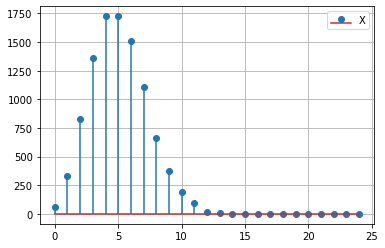
\includegraphics[width=\columnwidth]{poisson/solutions/1/Figures/FigureX.png}
    \caption{Poisson stem plot for X \brak{\lambda = 5}}
    \label{poisson/1/fig:plot1}
\end{figure}
\begin{figure}[hb]
    \centering
    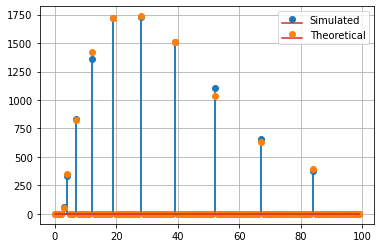
\includegraphics[width=\columnwidth]{poisson/solutions/1/Figures/FigureComp.png}
    \caption{Stem plot for Y (Simulated and Theoretical) \brak{\lambda = 5}}
    \label{poisson/1/fig:plot3}
\end{figure}




\end{enumerate}
%
\section{Gaussian  Distribution}
\renewcommand{\theequation}{\theenumi}
\renewcommand{\thefigure}{\theenumi}
\renewcommand{\thetable}{\theenumi}
\begin{enumerate}[label=\thesection.\arabic*.,ref=\thesection.\theenumi]
\numberwithin{equation}{enumi}
\numberwithin{figure}{enumi}
\numberwithin{table}{enumi}

\item Let $U$ and $V$ be two independent zero mean Gaussian random variables of variances $\frac{1}{4}$ and $\frac{1}{9}$ respectively. The probability $\pr{3V \geq 2U}$ is \dots
\\
\solution
From the given information,
\begin{align}
    U &= \gauss{0}{\frac{1}{4}}
    V &= \gauss{0}{\frac{1}{9}}
\end{align}
%
Let $Y = 3V - 2U$.  Then, 
\begin{align}
   \mean{Y} &= 3\mean{V} - 2\mean{U} = 0
\\
\var{Y} &= 3^2\var{V} + 2^2\var{U} = 2
\end{align}
\begin{align}
    \therefore Y = \gauss{0}{2}
\end{align}
Thus, 
\begin{align}
    \pr{3V \geq 2U} &= \pr{3V-2U \geq 0}
    \\
    &= \pr{Y \geq 0} = \frac{1}{2}
\end{align}
$\because$ Y is symmetric about the origin.

%
\item $(X,Y)$ follows bivariate normal distribution $N_2$(0,0,1,1,$\rho$),  -1 $<$ $\rho$ $<$ 1. Then,
\begin{enumerate}
    \item $X+Y$ and $X-Y$ are uncorrelated only if $\rho$ = 0
    \item $X+Y$ and $X-Y$ are uncorrelated only if $\rho$ $<$ 0
    \item $X+Y$ and $X-Y$ are uncorrelated only if $\rho$ $>$ 0
    \item $X+Y$ and $X-Y$ are uncorrelated for all values of $\rho$
\end{enumerate}
\solution
Given that 
\begin{align}
 \vec{M} = \myvec{ X \\ Y}
 \sim  \gauss{\boldsymbol{\upmu}}{\boldsymbol{\Sigma}}
\end{align}
%
where 
%Here, Mean matrix of X and Y is:
\begin{align}
    \boldsymbol{\upmu} &= \myvec{0 \\ 0}
    \\
\boldsymbol{\Sigma} &= \myvec{
            1 & \rho\\
            \rho & 1 
        }
\end{align}
Also, 
\begin{align}
    X+Y &
    = \vec{A}^\top \vec{M}
    \\
    X-Y &
    =\vec{B}^\top \vec{M}
\end{align}
where
\begin{align}
 \vec{A} &= \myvec{1 \\ 1}, 
    \vec{B} &= \myvec{1 \\ -1}
\end{align}
% Defining Covariance in terms of expectation value:
% \begin{align}
%     Cov(X,Y)=& E[(X-\boldsymbol{\upmu}_x)(Y-\boldsymbol{\upmu}_y)] \\
%     =& E[(X-0)(Y-0)]\\
%     =& E(XY)
% \end{align}
Thus, 
\begin{align}
 Cov(X+Y,X-Y) =& \vec{A}^\top \boldsymbol{\Sigma} \vec{B} \\
    % =& \myvec{1 \\ 1}^\top
    % \myvec{
    %         1 & \rho\\
    %         \rho & 1 
    %     }
    %     \myvec{1 \\ -1}\\ 
    % =& \myvec{1+\rho \\ 1+\rho}^\top
    %     \myvec{1 \\ -1}\\
    % =& (1+\rho)-1(1+\rho) \\
    =&   0
\end{align}
% Note that 
% \begin{align}
% Var(X+Y) = Cov(X+Y , X+Y)\\ 
%  Var(X-Y)  = Cov(X-Y , X-Y)
% \end{align}
% Hence,
% \begin{align}
%     Var(X+Y) =&\vec{A^\top} \boldsymbol{\Sigma} \vec{A} \\
%         =& \myvec{1 \\ 1}^\top
%          \myvec{
%             1 & \rho\\
%             \rho & 1 
%         }
%         \myvec{1 \\ 1}\\
%     =& \myvec{1+\rho \\ 1+\rho}^\top
%         \myvec{1 \\ 1}\\
%     =& 1+\rho+1+\rho \\
%     =& 2+2\rho \neq 0
% \end{align}
% \begin{align}
%     Var(X-Y) =& \vec{B^\top} \boldsymbol{\Sigma} \vec{B} \\
%         =& \myvec{1 \\ -1}^\top
%     \myvec{
%             1 & \rho\\
%             \rho & 1 
%         }
%          \myvec{1 \\ -1}\\
%     =& \myvec{1-\rho \\ \rho-1}^\top
%         \myvec{1 \\ -1}\\
%     =& 1-\rho-\rho+1 \\
%     =& 2-2\rho \neq 0
% \end{align}
% So correlation coefficient is:
% \begin{align}
%     \rho(X+Y,X-Y) = \frac{Cov(X+Y,X-Y)}{\sqrt{var(X+Y) \times var(X-Y)}}
%     = 0
% \end{align}
$\therefore$ X+Y and X-Y are uncorrelated irrespective of value of $\rho$ where $\rho \in \brak{-1,1}$.
%$\therefore$ The correct answer is \textbf{option 4}.
\end{enumerate}
%

\section{Geometric Distribution}
\renewcommand{\theequation}{\theenumi}
\renewcommand{\thefigure}{\theenumi}
\renewcommand{\thetable}{\theenumi}
\begin{enumerate}[label=\thesection.\arabic*.,ref=\thesection.\theenumi]
\numberwithin{equation}{enumi}
\numberwithin{figure}{enumi}
\numberwithin{table}{enumi}


\item Suppose $X$ has density 
%
\begin{align}
f\brak{x|\theta} = \frac{1}{\theta}e^{-x/\theta}, x>0 
\end{align}
Define 
\begin{align}
    Y=k, \quad k\leq X< k+1, \quad k=0,1,2\ldots
\end{align}
%
Then the distribution of $Y$ is
\begin{enumerate}
\begin{multicols}{2}
\setlength\itemsep{0.5em}
    \item Normal
    \item Binomial
    \item Poisson
    \item Geometric
\end{multicols}
\end{enumerate}
\solution
\begin{align}
    \pr{Y=k} &= \pr{k\leq X < k+1}\\
    &= \int_k^{k+1}f\brak{x|\theta}dx\\
    &= \int_k^{k+1}\frac{1}{\theta}e^{-\frac{x}{\theta}}dx\\
    &= \sbrak{-e^{-\frac{x}{\theta}}}_k^{k+1}\\
 &= e^{-\frac{k}{\theta}}\brak{1-e^{-\frac{1}{\theta}}}
 \\
 \implies     \pr{Y=k} &= \brak{1-p}^k p \, k=0,1,2\ldots
\end{align}
%
where
\begin{align}
    p=1-e^{-\frac{1}{\theta}}
\end{align}
Therefore, the distribution of $Y$ is 4) Geometric.




\end{enumerate}



\section{Two Dimensions}
\renewcommand{\theequation}{\theenumi}
\renewcommand{\thefigure}{\theenumi}
\renewcommand{\thetable}{\theenumi}
\begin{enumerate}[label=\thesection.\arabic*.,ref=\thesection.\theenumi]
\numberwithin{equation}{enumi}
\numberwithin{figure}{enumi}
\numberwithin{table}{enumi}

\item Let $ c \in \mathbb{R} $ be a constant. Let $ X, Y$ be random variables with joint probability density function 
\begin{align}
f(x,y)  = 
\begin{cases}
cxy &  0<x<y<1,
\\
0 & \text{ otherwise }
\end{cases}
\label{eq:: joint_pdf}
\end{align}
Which of the following statements are correct ?
\begin{enumerate}
    \item $c = \frac{1}{8}$
    \item $ c= 8$
    \item $X $ and $ Y$ are independent
    \item $\Pr\brak{X= Y} = 0 $
\end{enumerate}
\solution
\begin{enumerate}
    \item False
    \item By definition, 
    \begin{align}
        f_Y\brak{y} &=  \int_{-\infty}^{\infty} f(x,y) \,dx \\
        &= \int_{0}^{y} cxy \,dx \\
        &= cy \brak{\frac{x^2}{2}} \Biggr|_{0}^{y} \\
        &= \frac{ cy^3}{2}
    \end{align}
     \begin{align}
    \label{eq:: pdfy}
    \implies f_Y(y)  = 
    \begin{cases}
    \frac{ cy^3}{2}, &  0<y<1
    \\
    0 & \text{ otherwise. }
    \end{cases}
    \end{align}   
    $\because$ the area under the pdf is 1,  from \eqref{eq:: pdfy},
    \begin{align}
    \implies    \int_{-\infty}^{\infty} f_Y(y) \,dy &= 1 \\
    \implies        \int_{0}^{1} c\frac{y^3}{2} & =1 \\
    \implies    \frac{c}{8} &= 1 \\
    \text{or, }    c & = 8
    \end{align}
%
Also,
% The pdf of Y is 
 \begin{align}
\label{eq:: pdf_y}
f_Y(y)  = 
\begin{cases}
 4y^3 & \text{, if } 0<y<1
\\
0 & \text{, otherwise }
\end{cases}
\end{align}   

\item 
\begin{align}
    f_X\brak{x} &=  \int_{-\infty}^{\infty} f(x,y) \,dy \\
    &= \int_{x}^{1} cxy \,dy \\
    &= cx \brak{\frac{y^2}{2}} \Biggr|_{x}^{1} \\
    &= cx \brak{\frac{1- x^2}{2}}
\end{align}
%
\begin{align}
\label{eq:: pdf_x}
\implies f_X(x)  = 
\begin{cases}
4x \brak{1- x^2}, &  0<x<1
\\
0 & \text{ otherwise }
\end{cases}
\end{align} 
%
From \eqref{eq:: pdf_x} and \eqref{eq:: pdf_y}
\begin{align}
f_X(x) \times f_Y(y) & = 
\begin{cases}
16xy^3 \brak{1- x^2} & \text{, if } 0<x,y<1 
\\
0 & \text{, otherwise }
\end{cases}
\\
  &\neq f(x,y)
\end{align} 
%Since $f(x,y) $ and $ f_X(x) \times f_Y(y) $ are different, random variables 
Hence, $X$ and $Y$ are not independent. 
%Therefore option (3) is not correct. \\
\item
% The marginal PDF of X is given by,
% \begin{align}
% \label{eq:: pdf_x1}
% f_X(x)  = 
% \begin{cases}
% 4x \brak{1- x^2} & \text{, if } 0<x<1
% \\
% 0 & \text{, otherwise }
% \end{cases}
% \end{align} 
% The marginal CDF of X, $ F_X(x)$ is given by,
\begin{align}
    F_X(x) &=  \int_{-\infty}^{x} f_X(x) \,dx \\
    &= \int_{0}^{x} 4x(1-x^2) \,dx \\
     &= \int_{0}^{x} 4x-4x^3 \,dx \\
     & = 2x^2 - 4x^4 \text{ for }  0< x< 1
\end{align}
yielding
\begin{align}
\label{eq:: cdf_x}
F_X(x)  = 
\begin{cases}
0 &  x \le 0
\\
2x^2 - 4x^4    &  0 <x< 1
\\
1 &    x \ge 1
\end{cases}
\end{align}
From \eqref{eq:: cdf_x},
\begin{multline}
    \Pr\brak{Y- \epsilon < X < Y + \epsilon} 
    \\
    = F_X(Y + \epsilon) -  F_X(Y - \epsilon)  
    \\
     = 8\epsilon Y\brak{1 - Y^2 - \epsilon^2}
\end{multline}
upon simplification.  Letting
%
\begin{align}
g(Y)&= 8\epsilon Y(1 - Y^2 - \epsilon^2), \\
    E[g(Y)] &= \int_{-\infty}^{\infty} g(y) f_Y(y) \,dy 
    \\
     & = \int_{0}^{1} (4y^3) (8\epsilon y)(1 - y^2 - \epsilon^2) \,dy 
\end{align}
\begin{multline}
\implies     \Pr\brak{Y- \epsilon < X < Y + \epsilon}     \\
= 32\epsilon \brak{\frac{2- 7\epsilon^2}{35}}
\end{multline}
Now substituting $ \epsilon = 0 $ in the above, 
\begin{align}
    \pr{X =Y}  = 0
\end{align}
\end{enumerate}
%
\item Let $X$ and $Y$ be random variables having the joining probability density function
\begin{align}
f_{XY}(x,y)=
\begin{cases}
\frac{1}{\sqrt{2\pi y}}e^{\frac{-1}{2y}(x-y)^2} & 
\begin{array}{c}
x \in \brak{-\infty,\infty}, 
\\
y \in \brak{0, 1} 
\end{array}
\\
0 &\text{otherwise}
\end{cases}
\label{eq:twoD/2}
\end{align}
The covariance between the random variables X and Y is
\\
%
\solution
%The covariance is defined as
%
\begin{align}
    \cov{XY} = \mean{XY}-\mean{X}\mean{Y}
\end{align}
From \eqref{eq:twoD/2},
%
\begin{align}
    E\brak{XY}=&\int_{0}^{1}\int_{-\infty}^{\infty}xy f_{XY}(x,y)\,dx\,dy\\
    =&\int_{0}^{1}\int_{-\infty}^{\infty}xy\frac{1}{\sqrt{2\pi y}}e^{\frac{-1}{2y}(x-y)^2}\,dx \,dy\\
    =&\int_{0}^{1}y^2 \,dy\\
     \implies E\brak{XY}=&\frac{1}{3} \label{eq:1}
    \end{align}
Y has marginal probability
\begin{align}
    f_Y(y)=&\int_{-\infty}^{\infty}f_{XY}(x,y)\,dx =1\\
    \implies E\brak{Y}=&\frac{1}{2} \label{eq:2}
\end{align}
\begin{align}
 E\brak{X}=&\int_{0}^{1}\int_{-\infty}^{\infty}x f_{XY}(x,y)\,dx\,dy\\
    =&\int_{0}^{1}\int_{-\infty}^{\infty}x\frac{1}{\sqrt{2\pi y}}e^{\frac{-1}{2y}(x-y)^2}\,dx \,dy\\
    =&\int_{0}^{1}y\,dy\\
E\brak{X}=&\frac{1}{2} \label{eq:3} \\
\end{align}
From \eqref{eq:1},\eqref{eq:2},\eqref{eq:3}
\begin{align}
Cov(X,Y)=&E\brak{XY}-E\brak{X}E\brak{Y}\\
       =&\frac{1}{3}-\frac{1}{2}\times \frac{1}{2}\\
Cov(X,Y)=&\frac{1}{12}
\end{align}
\item Let a random variable $X$ follow exponential distribution with mean 2. Define $Y=[X-2|X>2]$. The value of $\pr{Y \geq t}$ is \dots
\\
%
\solution
%Given that, $Y=[X-2|X>2]$
From the given information, 
\begin{align}
\pr{Y \geq t} &= \frac{\pr{X-2 \geq t, X>2}}{\pr{X>2}} 
\\
&= \frac{\pr{X \geq t + 2, X>2}}{\pr{X>2}} 
\label{twoD/3/Eq:1}
\end{align}
$\because  X$ has an exponential distribution with parameter $\lambda = \frac{1}{2}$, 
\begin{align}
	F_X\brak{x} &= \begin{cases} \label{twoD/3/Eq:3}
				1 - e^{-\lambda x}, & \text{if $0 < x< \infty $}\\
				0, & \text{otherwise}
			 \end{cases} 
%	E\brak{x} &= \frac{1}{\lambda} \label{twoD/3/Eq:4}
	\end{align}
	and
	%
\begin{align}
	\pr{X >2} = 1- F_X\brak{2} = e^{-2\lambda}
	\label{twoD/3/Eq:7} 
	\end{align}
%	
Also, 
\begin{align}
	\label{twoD/3/Eq:6}
	\pr{X \geq t+2,X>2} &= 
	\begin{cases}
	\pr{X \geq t+2} & t \ge 0 \\
	\pr{X > 2} & t < 0	
	\end{cases}
		\end{align}
Substituting \eqref{twoD/3/Eq:6} in \eqref{twoD/3/Eq:1},  using 	\eqref{twoD/3/Eq:7} and simplifying,  
\begin{align}
\pr{Y \geq t} = 
\begin{cases}
	 e^{-\frac{t}{2}} & t \ge 0 \\
	1 & t < 0	
	\end{cases}
\end{align}

\end{enumerate}

\section{Markov Chain}
\renewcommand{\theequation}{\theenumi}
\renewcommand{\thefigure}{\theenumi}
\renewcommand{\thetable}{\theenumi}
\begin{enumerate}[label=\thesection.\arabic*.,ref=\thesection.\theenumi]
\numberwithin{equation}{enumi}
\numberwithin{figure}{enumi}
\numberwithin{table}{enumi}


\item \textbf{Step 1.} Flip a coin twice.\\
\textbf{Step 2.} If the outcomes are (TAILS, HEADS) then output Y and stop.\\
\textbf{Step 3.} If the outcomes are either (HEADS, HEADS) or (HEADS, TAILS), then output N and stop.\\
\textbf{Step 4.} If the outcomes are (TAILS, TAILS), then go to Step 1.\\
The probability that the output of the experiment is Y is (upto two decimal places)......
%
\solution
Given, a fair coin is tossed is tossed two times.
Let's define a Markov chain $\{X_{n},n=0,1,2,\dots\}$, where $X_{n}\in S=\{1,2,3\}$, such that
\begin{table}[h!]
\centering
\caption{States and their notations}
\label{ec9:table:1}
\begin{tabular}{|c|c|}
    \hline
    Notation & State \\
    \hline
    $S=1$ & getting \cbrak{TT}\\[1ex]
    \hline
    $S=2$ & getting output Y\\[1ex]
    \hline
    $S=3$ & getting output N\\[1ex]
    \hline
\end{tabular}
\end{table}\\
The state transition matrix for the Markov chain is
\begin{align}
\label{ec9:eq:1}
P=\begin{blockarray}{cccccc}
&1 & 2 & 3 \\
\begin{block}{c[ccccc]}
  1 & 0.25 & 0.25 & 0.5  \\
  2 & 0 & 1 & 0 \\
  3 & 0 & 0 & 1  \\
\end{block}
\end{blockarray}
\end{align}
Clearly, the state $1$ are transient, while $2,3$ are absorbing. The standard form of a state transition matrix is
\begin{align}
\label{ec9:eq:2}
P=\begin{blockarray}{ccc}
&A & N \\
\begin{block}{c[cc]}
  A & I & O  \\
  N & R & Q \\
\end{block}
\end{blockarray}
\end{align}
where,
\begin{table}[h!]
\centering
\caption{Notations and their meanings}
\label{ec9:table:2}
\begin{tabular}{|c|c|}
    \hline
    Notation & Meaning \\
    \hline
    $A$ & All absorbing states\\[1ex]
    \hline
    $N$ & All non-absorbing states\\[1ex]
    \hline
    $I$ & Identity matrix\\[1ex]
    \hline
    $O$ & Zero matrix\\[1ex]
    \hline
    $R,Q$ & Other submatices\\[1ex]
    \hline
\end{tabular}
\end{table}
Converting \eqref{ec9:eq:1} to standard form, we get
\begin{align}
P=\begin{blockarray}{cccccc}
&2 & 3 & 1  \\
\begin{block}{c[ccccc]}
  2 & 1 & 0 & 0  \\
  3 & 0 & 1 & 0 \\
  1 & 0.25 & 0.5 & 0.25  \\
\end{block}
\end{blockarray}
\end{align}
From \eqref{ec9:eq:2},
\begin{align}
\tag{104.5}
\label{ec9:eq:r,q}
    R=\begin{bmatrix}
    0.25 & 0.5\\
    \end{bmatrix},
    Q=\begin{bmatrix}
    0.25\\
    \end{bmatrix}
\end{align}
The limiting matrix for absorbing Markov chain is
\begin{align}
\bar P=\begin{bmatrix}
    I & O\\
    FR & O\\
    \end{bmatrix}
\end{align}
where,
\begin{align}
F=(I-Q)^{-1}
\end{align}
is called the fundamental matrix of $P$. \\
On solving, we get
\begin{align}
\bar P=\begin{blockarray}{cccccc}
&2 & 3 & 1 \\
\begin{block}{c[ccccc]}
    2 & 1 & 0 & 0\\ 
    3 & 0 & 1 & 0\\ 
    1 & 0.33 & 0.17 & 0\\    
\end{block}
\end{blockarray}
\end{align}
A element $\bar p_{ij}$ of $\bar P$ denotes the absorption probability in state $j$, starting from state $i$. 
\\ Then, the absorption probability in state 2 $\brak{\text{i.e getting output Y}}$ starting from state 1 is $\bar p_{12}$.
\begin{align}
\therefore \bar p_{12}=0.33 \brak{\text{correct upto 2 decimal places}}
\end{align}
\begin{figure}[h]
\caption*{\textbf{Markov chain diagram}}
\centering
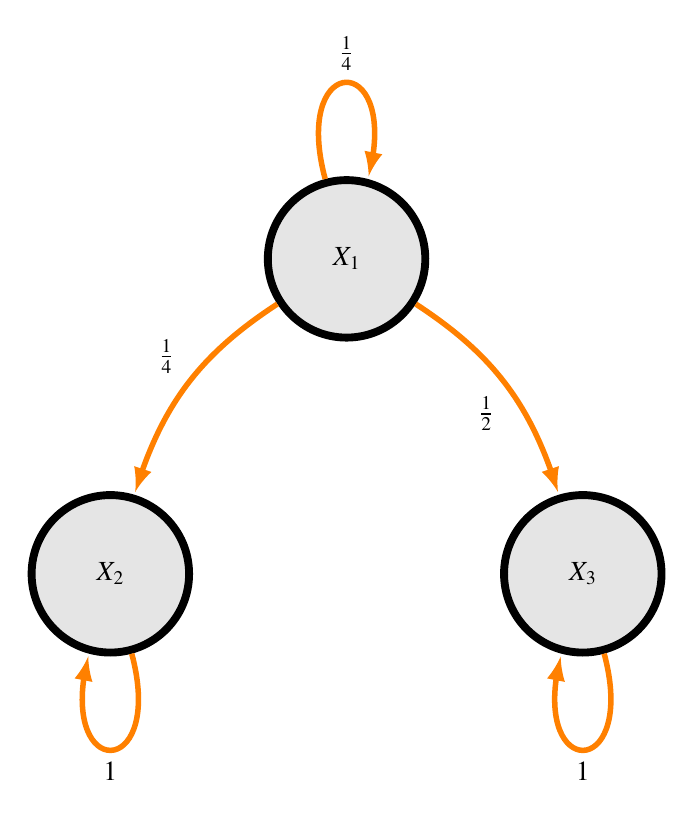
\begin{tikzpicture}
       
             % Setup the style for the states
        \tikzset{node style/.style={state, 
                                    minimum width=2cm,
                                    line width=1mm,
                                    fill=gray!20!white}}
        % Draw the states
        \node[node style] at (3, 0)      (bull)     {$X_{1}$};
        \node[node style] at (0, -4)      (bear)     {$X_{2}$};
        \node[node style] at (6, -4) (stagnant) {$X_{3}$};
        % Connect the states with arrows
        \draw[every loop,
              auto=right,
              line width=0.7mm,
              >=latex,
              draw=orange,
              fill=orange]
           (bull)     edge[bend left=20]            node {$\frac{1}{2}$} (stagnant)
            (bull)     edge[bend right=20] node {$\frac{1}{4}$} (bear)
            
            
            (bull) edge[loop above]             node  {$\frac{1}{4}$} (bull)
            (bear) edge[loop below]             node  {1} (bear)
            (stagnant) edge[loop below]             node  {1} (stagnant);
    \end{tikzpicture}
\end{figure}


\end{enumerate}

%
\section{Convergence}
\renewcommand{\theequation}{\theenumi}
\renewcommand{\thefigure}{\theenumi}
\renewcommand{\thetable}{\theenumi}
\begin{enumerate}[label=\thesection.\arabic*.,ref=\thesection.\theenumi]
\numberwithin{equation}{enumi}
\numberwithin{figure}{enumi}
\numberwithin{table}{enumi}
%
\item 
Let $X_{1},X_{2},\dots$ be independent and identically distributed random variables each following a uniform distribution on (0,1). Denote 
\begin{align}
T_{n}=\max\cbrak{ X_{1},X_{2},\dots,X_{n}}. 
\end{align}
Then, which of the following statements are true?
\begin{enumerate}
    \item $T_{n}$ converges to 1 in probability.
    \item $n(1-T_{n})$ converges in distribution.
    \item $n^{2}(1-T_{n})$ converges in distribution.
    \item $\sqrt{n}(1-T_{n})$ converges to 0 in probability.
\end{enumerate}
%
\solution
\begin{definition}
{\em Random Sampling :}
A collection of random variables $X_{1},X_{2},\dots,X_{n}$ is said to be a random sample of size $n$ if they are independent and identically distributed, i.e,
\begin{enumerate}
    \item $X_{1},X_{2},\dots,X_{n}$ are independent random variables
    \item They have the same distribution (Let us denote it by $F_{X}(x)$), i.e,
    \begin{align}
        F_{X}(x)=F_{X_{i}}(x), i = 1,2,\dots,n \forall x\in \mathbb{R}
    \end{align}
\end{enumerate}
\end{definition}
\begin{definition}
{\em Order Statistics :}
Given a random sample $X_{1},X_{2},\dots,X_{n}$, the sequence $X_{(1)},X_{(2)},\dots,X_{(n)}$ is called the order statistics of it. Here,
\begin{align}
    &X_{(1)}=\min\brak{X_{1},X_{2},\dots,X_{n}}\\
    &X_{(2)}=\text{the }2^{nd}\text{ smallest of }X_{1},X_{2},\dots,X_{n}\\
    &\vdots\\
    &X_{(n)}=\max\brak{X_{1},X_{2},\dots,X_{n}}
\end{align}
\end{definition}
\begin{lemma}
{\em Distribution of the maximum :}
\begin{align}
	\label{eq:conv/1/pdf}
    f_{T_{n}}(x)&=\begin{cases}
	nx^{n-1}, & 0< x<1 \\~\\[-1em]
	0, & otherwise
	\end{cases}\\
	F_{T_{n}}(x)&=\begin{cases}
	x^{n}, & 0< x<1 \\~\\[-1em]
	1, & x\geq 1\\~\\[-1em]
	0, & otherwise
	\end{cases} 
	\label{eq:conv/1/cdf}
\end{align}
\end{lemma}
%\proof
Proof:
\begin{align}
   F_{X_{(n)}}(x)&=\pr{X_{(n)}\leq x}\\
   &=\pr{X_{1}\leq x,X_{2}\leq x,\dots,X_{n}\leq x}\\
   &=\pr{X_{1}\leq x}\pr{X_{2}\leq x}\dots\pr{X_{n}\leq x}\\
   \label{conv/1/eq:F}
   &=\sbrak{\pr{X_{1}\leq x}}^{n}\brak{ \text{i.i.d}}\\
   &=\sbrak{F_{X}(x)}^{n}
   \label{eq:conv/1/cdf/max}
\end{align}
and 
\begin{align}
   f_{X_{(n)}}(x)&=\dfrac{d}{dx}\brak{F_{X_{(n)}}(x)}=\dfrac{d}{dx}\brak{\sbrak{F_{X}(x)}^{n}}\\
   &=n\brak{\sbrak{F_{X}(x)}^{n-1}}\dfrac{d}{dx}\brak{F_{X}(x)}\\
%   \label{conv/1/eq:f}
   &=n\sbrak{F_{X}(x)}^{n-1}f_{X}(x)
   \label{eq:conv/1/pdf/max}
\end{align}
$\because $
\begin{align}
    f_{X_{i}}(x)&=\begin{cases}
	1, & 0< x<1 \\~\\[-1em]
	0, & otherwise
	\end{cases},
	\\
	F_{X_{i}}(x)&=\begin{cases}
	x, & 0< x<1 \\~\\[-1em]
	1, & x\geq 1\\~\\[-1em]
	0, & otherwise,
	\end{cases} 
\end{align}
$\forall i\in \mathbb{N}$.  Substituting the above in    \eqref{eq:conv/1/pdf/max} and \eqref{eq:conv/1/cdf/max} yields 	\eqref{eq:conv/1/pdf} and 	\eqref{eq:conv/1/cdf} respectively. 
Then, as $T_{n}=max\{ X_{1},X_{2},\dots,X_{n}\}=X_{(n)}$,
\begin{lemma}
If $Y=aX+b$ and $a<0$, then
\begin{align}
\label{conv/1/eq:form}
    F_{Y}(y)=1-F_{X}\brak{\dfrac{y-b}{a}}
\end{align}
\end{lemma}
\begin{definition}
{\em	Convergence in Probability :}
A sequence of random variables $X_{1},X_{2},X_{3},\dots$ converges in probability to a random variable $X$, shown by $X_{n}\xrightarrow[]{p}X$, if
\begin{align}
    \displaystyle\lim_{n\to\infty}\pr{|X_{n}-X|\geq\epsilon}=0,\forall\epsilon>0
\end{align}
\end{definition}
%
\begin{definition}
	{\em Convergence in Distribution :}
A sequence of random variables $X_{1},X_{2},X_{3},\dots$ converges in distribution to a random variable $X$, shown by $X_{n}\xrightarrow[]{d}X$, if
\begin{align}
    \displaystyle\lim_{n\to\infty}F_{X_{n}}(x)=F_{X}(x)
\end{align}
for all $x$ at which $F_{X}(x)$ is continuous.
\end{definition}
%
\begin{enumerate}
\item 
%To evaluate : $\displaystyle\lim_{n\to\infty}\pr{|T_{n}-1|\geq\epsilon},\forall\epsilon>0$
\begin{multline}
    \displaystyle\lim_{n\to\infty}\pr{|T_{n}-1|\geq\epsilon}=\displaystyle\lim_{n\to\infty}\pr{1-T_{n}\geq\epsilon}\\
	=\displaystyle\lim_{n\to\infty}\pr{T_{n}\leq1-\epsilon}=\displaystyle\lim_{n\to\infty}F_{T_{n}}(1-\epsilon)
	\label{conv/1/1/cdf}
\end{multline}
\begin{align}
    \because F_{T_{n}}(1-\epsilon)=\begin{cases}
	(1-\epsilon)^{n}, & 0< \epsilon<1 \\~\\[-1em]
	0, & \epsilon\geq 1
	\end{cases}
	\label{conv/1/1/cdf/epsilon}
\end{align}
and 
\begin{align}
	\label{conv/1/1/cdf/epsilon/lim}
    \because\displaystyle\lim_{n\to\infty}(1-\epsilon)^{n}=0 \text{ for } 0< \epsilon<1\\
\end{align}
%
from 	\eqref{conv/1/1/cdf/epsilon/lim}, 	\eqref{conv/1/1/cdf/epsilon} and 	\eqref{conv/1/1/cdf},
\begin{align}
	 \displaystyle\lim_{n\to\infty}\pr{|T_{n}-1|\geq\epsilon}=0,\forall\epsilon>0
\end{align}
$\therefore T_{n}$ converges to 1 in probability.
\item 
Substituting $a=-n,b=n$ in \eqref{conv/1/eq:form},
\begin{align}
	F_{n(1-T_{n})}(x)=1-F_{T_{n}}\brak{1-\dfrac{x}{n}}\\
\end{align}	
where
\begin{align}
    F_{T_{n}}\brak{1-\dfrac{x}{n}}=\begin{cases}
	\brak{1-\dfrac{x}{n}}^{n}, & 0< x<n \\~\\[-1em]
	1, & x\leq 0\\~\\[-1em]
	0, & x\geq n
	\end{cases} \\
	from  	\eqref{eq:conv/1/cdf}
\end{align}
\begin{align}
	\because\displaystyle\lim_{n\to\infty}\brak{1-\dfrac{y}{n}}^{n}=e^{-y}, \\
\end{align}
\begin{align}
\therefore\displaystyle\lim_{n\to\infty} F_{T_{n}}\brak{1-\dfrac{x}{n}}&=\begin{cases}
	e^{-x}, & x>0 \\~\\[-1em]
	1, & x\leq 0
	\end{cases} \\
	\implies 
	\displaystyle\lim_{n\to\infty}F_{n(1-T_{n})}(x)&=1-\displaystyle\lim_{n\to\infty} F_{T_{n}}\brak{1-\dfrac{x}{n}}
\end{align}
which can be expressed as
\begin{align}
\label{conv/1/eq:cdf1}
    \therefore\displaystyle\lim_{n\to\infty} F_{n(1-T_{n})}(x)=\begin{cases}
	1-e^{-x}, & x>0 \\~\\[-1em]
	0, & x\leq 0
	\end{cases} 
\end{align}
$\therefore n(1-T_{n})$ converges in distribution to the random variable $X\sim Exponential(1)$.
% \begin{figure}[h!]
% \centering
% \includegraphics[width=\linewidth]{Assignment9}
% \caption{CDF}
% \label{conv/1/plot}
% \end{figure}
\item 
Substituting $a=-n^{2},b=n^{2}$ in \eqref{conv/1/eq:form},
\begin{align}
    F_{n^{2}(1-T_{n})}(x)&=1-F_{T_{n}}\brak{1-\dfrac{x}{n^{2}}}\\
    F_{T_{n}}\brak{1-\dfrac{x}{n^{2}}}&=\begin{cases}
	\brak{1-\dfrac{x}{n^{2}}}^{n}, & 0< x<n^{2} \\~\\[-1em]
	1, & x\leq 0\\~\\[-1em]
	0, & x\geq n^{2}
	\end{cases} \\
	&=\begin{cases}
		1, & x>0 \\~\\[-1em]
		1, & x\leq 0
		\end{cases} 
	\end{align}
	\begin{align}
	\because\displaystyle\lim_{n\to\infty}\brak{1-\dfrac{x}{n^{2}}}^{n}=1
%&\therefore\displaystyle\lim_{n\to\infty} F_{T_{n}}\brak{1-\dfrac{x}{n^{2}}}
	\end{align}
	yielding 
	\begin{align}
%&\because\displaystyle\lim_{n\to\infty}F_{n^{2}(1-T_{n})}(x)=1-\displaystyle\lim_{n\to\infty} F_{T_{n}}\brak{1-\dfrac{x}{n^{2}}}\\
\label{conv/1/eq:cdf2}
    \displaystyle\lim_{n\to\infty} F_{n^{2}(1-T_{n})}(x)=\begin{cases}
	0, & x>0 \\~\\[-1em]
	0, & x\leq 0
	\end{cases} 
\end{align}
which is not a valid CDF.  Hence, 
%$\because$ The CDF in \eqref{conv/1/eq:cdf2} is not valid,\\
$ n^{2}(1-T_{n})$ does not converge in distribution.
\item 
% Convergence in Probability :\\
% A sequence of random variables $X_{1},X_{2},X_{3},\dots$ converges in probability to a random variable $X$, shown by $X_{n}\xrightarrow[]{p}X$, if
% \begin{align}
%     \displaystyle\lim_{n\to\infty}\pr{|X_{n}-X|\geq\epsilon}=0,\forall\epsilon>0
% \end{align}
% To evaluate :\\ $\displaystyle\lim_{n\to\infty}\pr{|\sqrt{n}(1-T_{n})-0|\geq\epsilon},\forall\epsilon>0$
\begin{multline}
	\displaystyle\lim_{n\to\infty}\pr{|\sqrt{n}(1-T_{n})-0|\geq\epsilon}    \\ =\displaystyle\lim_{n\to\infty}\pr{1-T_{n}\geq\dfrac{\epsilon}{\sqrt{n}}}\\
    =\displaystyle\lim_{n\to\infty}\pr{T_{n}\leq1-\dfrac{\epsilon}{\sqrt{n}}}\\
	=\displaystyle\lim_{n\to\infty}F_{T_{n}}\brak{ 1-\dfrac{\epsilon}{\sqrt{n}}}
	\\
	=\begin{cases}
		\brak{1-\dfrac{\epsilon}{\sqrt{n}}}^{n}, & 0< \epsilon< \sqrt{n}\\~\\[-1em]
		0, & \epsilon\geq \sqrt{n}
		\end{cases}
\end{multline}
\begin{multline}
%    &F_{T_{n}}\brak{1-\dfrac{\epsilon}{\sqrt{n}}}\\
    \because\displaystyle\lim_{n\to\infty}\brak{1-\dfrac{\epsilon}{\sqrt{n}}}^{n}=0 \text{ for } 0< \epsilon<\sqrt{n},\\
     \displaystyle\lim_{n\to\infty}\pr{|\sqrt{n}(1-T_{n})-0|\geq\epsilon}=0,\forall\epsilon>0
\end{multline}
$\therefore\sqrt{n}(1-T_{n})$ converges to 0 in probability.
\end{enumerate}
\begin{lstlisting}
Hence, options 1), 2), 4) are correct.
\end{lstlisting}
%
\item Let $\{X_i\}_{i \geq 1}$ be a sequence of i.i.d. random variables with $E(X_i)=0$ and $V(X_i)=1$. Which of the following are true?
%
\begin{enumerate}
    \setlength{\itemsep}{2pt}
    \item $\dfrac{1}{n} \sum_{i=1}^n X_i^2 \to 0$ in probability 
    \item $\dfrac{1}{n^{3/4}} \sum_{i=1}^n X_i \to 0$ in probability 
    \item $\dfrac{1}{n^{1/2}} \sum_{i=1}^n X_i \to 0$ in probability 
    \item $\dfrac{1}{n} \sum_{i=1}^n X_i^2 \to 1$ in probability
\end{enumerate}
%
\solution
        \begin{lemma}
            {\em Strong Law of Large Numbers: }
            Let $X_1, X_2, \cdot \cdot \cdot$ be a sequence of i.i.d. random variables, each having finite mean $E(X_i)$. Then for any $\epsilon >0$,
            \begin{align}
                \lim_{n \to \infty}\pr{\left|\dfrac{1}{n}\sum_{i=1}^nX_i - E(X_i)\right|\geq \epsilon}=0
            \end{align}
            Or, $\frac{1}{n}\sum_{i=1}^nX_i$ converges in probability to $E(X_i)$.
        \end{lemma}

%
\item Let $X_1,X_2, \dots$ be i.i.d. $N(0,1)$ random variables. Let 
\begin{align}
S_{n}=X_{1}^2+X_{2}^2+\dots+X_{n}^2 \forall n \geq 1. 
\end{align}
Which of the following statements are correct?
%
\begin{enumerate}
\setlength\itemsep{1em}
\item 
\begin{align}
    \frac{S_{n}-n}{\sqrt{2}}\sim N(0,1) \quad  \forall n\geq 1
\end{align}
\item 
\begin{align}
    \forall \epsilon > 0,\pr{\abs{\frac{S_n}{n}-2}>\epsilon}\to 0, n \to \infty
\end{align}

\item $\frac{S_{n}}{n} \to 1$ with probability 1
\item 
\begin{multline}
    \pr{{S_{n} \leq n+\sqrt{n}x}} \to \pr{{Y \leq x}}
    \\
    \forall x\in \mathbb{R}, Y \sim N\brak{0,2}
\end{multline}
%
\end{enumerate}


%
\end{enumerate}
%
%
\section{Statistics}
\renewcommand{\theequation}{\theenumi}
\renewcommand{\thefigure}{\theenumi}
\renewcommand{\thetable}{\theenumi}
\begin{enumerate}[label=\thesection.\arabic*.,ref=\thesection.\theenumi]
\numberwithin{equation}{enumi}
\numberwithin{figure}{enumi}
\numberwithin{table}{enumi}



\item Let $Y_1$ denote the first order statistic in a random sample of size $n$ from a distribution that has the pdf 
\begin{align}
    f(x) = 
    \begin{cases}
    e^{-(x-\theta)}&\text{ when } \theta<x<\infty\\
    0 &\text{  otherwise} 
    \end{cases}
\end{align}
Obtain the distribution of $Z_n = n(Y_1 - \theta)$.
%
\\
\solution
From the given information
\begin{align}
    Y_1 = \min\{X_1, X_2, ... X_n\}
\end{align}
%
and
\begin{align}
    F_{Z_n}(z) &= \pr{n(Y_1-\theta)\leq z}\\
    &= \pr{Y_1\leq \frac{z}{n} +\theta}\\
    &= 1-\pr{Y_1\ > \frac{z}{n} +\theta}\label{stats/1/eq_2}
\end{align}
%
Let
\begin{align}
    \brak{\dfrac{z}{n}+\theta} = z^{\prime}
\end{align}
%
Then
\begin{align}
    F_{Z_n}\brak{z}    &= 1-\prod_{i=1}^{n}\pr{X_i>z^{\prime}}\\
    &= 1-\brak{1-F(z^{\prime})}^n\\
    \implies F_{Z_n}(z) &= 1-\brak{1-F\brak{\frac{z}{n}+\theta}}^n\label{stats/1/eq_3}
\end{align}
%
where
%
\begin{align}
  F(x) &=\displaystyle\int\limits_{-\infty}^{x} f(t) \,dt\\
&=
    \begin{cases}
    1-e^{-(x-\theta)} &\text{when }\theta<x<\infty\\
    0 &\text{otherwise}
    \end{cases}
    \label{stats/1/eq_1}
\end{align}
%
Substituting from     \eqref{stats/1/eq_1} in \eqref{stats/1/eq_3},
\begin{align}
    F_{Z_n}(z) &=
    \begin{cases}
    1-e^{-n\brak{\frac{z}{n}+\theta-\theta}}&  \theta<\frac{z}{n}+\theta<\infty\\
    0&\text{otherwise}
    \end{cases}\\
    &= \begin{cases}
    1-e^{-z}&\text{when } 0<z<\infty\\
    0 &\text{otherwise}\label{stats/1/cdf}
    \end{cases}
\end{align}
and 
\begin{align}
    f_{Z_n}(z) &= \frac{d}{dz}F_{Z_n}(z)\\
    &=\begin{cases}
    e^{-z}& 0<z<\infty\\
    0&\text{otherwise}
    \end{cases}\label{stats/1/pdf}
\end{align}
The plots for the cdf in \eqref{stats/1/cdf} and the pdf in \eqref{stats/1/pdf} are shown in Fig. \ref{stats/1/fig_cdf} and Fig. \ref{stats/1/fig_pdf} respectively:
\begin{figure}[!ht]
    \centering
    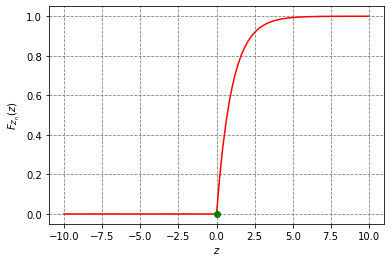
\includegraphics[width=\columnwidth]{stats/solutions/1/figures/cdf.png}
    \caption{cdf of $Z_n$}
    \label{stats/1/fig_cdf}
\end{figure}
\begin{figure}[!ht]
    \centering
    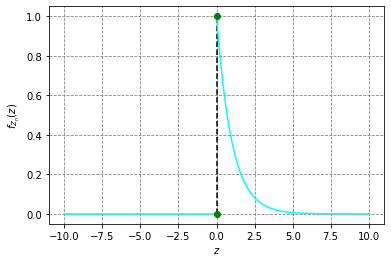
\includegraphics[width=\columnwidth]{stats/solutions/1/figures/pdf.png}
    \caption{pdf of $Z_n$}
    \label{stats/1/fig_pdf}
\end{figure}





\end{enumerate}
% \section{Unsolved Problems}
% \renewcommand{\theequation}{\theenumi}
\renewcommand{\thefigure}{\theenumi}
\renewcommand{\thetable}{\theenumi}
\begin{enumerate}[label=\thesection.\arabic*.,ref=\thesection.\theenumi]
\numberwithin{equation}{enumi}
\numberwithin{figure}{enumi}
\numberwithin{table}{enumi}


\item Which of the following conditions imply independence of the random variables $X$
and $Y$ ?\\
\begin{enumerate}
    \item  $\pr{X\ \mathop{>}\ a|Y\ \mathop{>}\ a} = \pr{X\ \mathop{>}\ a}\ \forall\ a\ \in\ \mathbb{R}$\\ 
    \item  $\pr{X\ \mathop{>}\ a|Y\ \mathop{<}\ b} = \pr{X\ \mathop{>}\ a}\ \forall\ a,\ b\ \in\ \mathbb{R}$\\ 
    \item  $X$ and $Y$ are uncorrelated.\\
    \item  $E[(X-a)(Y-b)] = E(X-a)\ E(Y-b)\ \forall\ a,\ b \in\ \mathbb{R}$\\
\end{enumerate}

\end{enumerate}

%  \section{June 2019}
%  \input{./chapters/2019.tex}
% \section{December 2018}
% \input{./chapters/2018/dec.tex}
% \section{June 2018}
% \input{./chapters/2018/june.tex}
% \section{December 2017}
% \input{./chapters/2017/dec.tex}
% %\twocolumn
% \section{June 2017}
% \input{./chapters/2017/june.tex}
% \section{December 2016}
% \input{./chapters/2016/dec.tex}
% \section{June 2016}
% \input{./chapters/2016/june.tex}
% \section{December 2015}
% \input{./chapters/2015/dec.tex}
% \section{June 2015}
% \input{./chapters/2015/june.tex}
%  \section{December 2014}
%  \input{./chapters/2014/dec.tex}
% \section{June 2013}
% \input{./chapters/2013/june.tex}

% \section{December 2012}
% \input{./chapters/2012/dec.tex}

% \section{June 2012}
% \input{./chapters/2012/june.tex}


\end{document}


